%% bare_conf_compsoc.tex
%% V1.4b
%% 2015/08/26
%% by Michael Shell
%% See:
%% http://www.michaelshell.org/
%% for current contact information.
%%
%% This is a skeleton file demonstrating the use of IEEEtran.cls
%% (requires IEEEtran.cls version 1.8b or later) with an IEEE Computer
%% Society conference paper.
%%
%% Support sites:
%% http://www.michaelshell.org/tex/ieeetran/
%% http://www.ctan.org/pkg/ieeetran
%% and
%% http://www.ieee.org/

%%*************************************************************************
%% Legal Notice:
%% This code is offered as-is without any warranty either expressed or
%% implied; without even the implied warranty of MERCHANTABILITY or
%% FITNESS FOR A PARTICULAR PURPOSE! 
%% User assumes all risk.
%% In no event shall the IEEE or any contributor to this code be liable for
%% any damages or losses, including, but not limited to, incidental,
%% consequential, or any other damages, resulting from the use or misuse
%% of any information contained here.
%%
%% All comments are the opinions of their respective authors and are not
%% necessarily endorsed by the IEEE.
%%
%% This work is distributed under the LaTeX Project Public License (LPPL)
%% ( http://www.latex-project.org/ ) version 1.3, and may be freely used,
%% distributed and modified. A copy of the LPPL, version 1.3, is included
%% in the base LaTeX documentation of all distributions of LaTeX released
%% 2003/12/01 or later.
%% Retain all contribution notices and credits.
%% ** Modified files should be clearly indicated as such, including  **
%% ** renaming them and changing author support contact information. **
%%*************************************************************************


% *** Authors should verify (and, if needed, correct) their LaTeX system  ***
% *** with the testflow diagnostic prior to trusting their LaTeX platform ***
% *** with production work. The IEEE's font choices and paper sizes can   ***
% *** trigger bugs that do not appear when using other class files.       ***                          ***
% The testflow support page is at:
% http://www.michaelshell.org/tex/testflow/



\documentclass[conference,compsoc]{IEEEtran}
% Some/most Computer Society conferences require the compsoc mode option,
% but others may want the standard conference format.
%
% If IEEEtran.cls has not been installed into the LaTeX system files,
% manually specify the path to it like:
% \documentclass[conference,compsoc]{../sty/IEEEtran}





% Some very useful LaTeX packages include:
% (uncomment the ones you want to load)


% *** MISC UTILITY PACKAGES ***
%
%\usepackage{ifpdf}
% Heiko Oberdiek's ifpdf.sty is very useful if you need conditional
% compilation based on whether the output is pdf or dvi.
% usage:
% \ifpdf
%   % pdf code
% \else
%   % dvi code
% \fi
% The latest version of ifpdf.sty can be obtained from:
% http://www.ctan.org/pkg/ifpdf
% Also, note that IEEEtran.cls V1.7 and later provides a builtin
% \ifCLASSINFOpdf conditional that works the same way.
% When switching from latex to pdflatex and vice-versa, the compiler may
% have to be run twice to clear warning/error messages.






% *** CITATION PACKAGES ***
%
\ifCLASSOPTIONcompsoc
  % IEEE Computer Society needs nocompress option
  % requires cite.sty v4.0 or later (November 2003)
  \usepackage[nocompress]{cite}
\else
  % normal IEEE
  \usepackage{cite}
\fi
% cite.sty was written by Donald Arseneau
% V1.6 and later of IEEEtran pre-defines the format of the cite.sty package
% \cite{} output to follow that of the IEEE. Loading the cite package will
% result in citation numbers being automatically sorted and properly
% "compressed/ranged". e.g., [1], [9], [2], [7], [5], [6] without using
% cite.sty will become [1], [2], [5]--[7], [9] using cite.sty. cite.sty's
% \cite will automatically add leading space, if needed. Use cite.sty's
% noadjust option (cite.sty V3.8 and later) if you want to turn this off
% such as if a citation ever needs to be enclosed in parenthesis.
% cite.sty is already installed on most LaTeX systems. Be sure and use
% version 5.0 (2009-03-20) and later if using hyperref.sty.
% The latest version can be obtained at:
% http://www.ctan.org/pkg/cite
% The documentation is contained in the cite.sty file itself.
%
% Note that some packages require special options to format as the Computer
% Society requires. In particular, Computer Society  papers do not use
% compressed citation ranges as is done in typical IEEE papers
% (e.g., [1]-[4]). Instead, they list every citation separately in order
% (e.g., [1], [2], [3], [4]). To get the latter we need to load the cite
% package with the nocompress option which is supported by cite.sty v4.0
% and later.





% *** GRAPHICS RELATED PACKAGES ***
%
\ifCLASSINFOpdf
  % \usepackage[pdftex]{graphicx}
  % declare the path(s) where your graphic files are
  % \graphicspath{{../pdf/}{../jpeg/}}
  % and their extensions so you won't have to specify these with
  % every instance of \includegraphics
  % \DeclareGraphicsExtensions{.pdf,.jpeg,.png}
\else
  % or other class option (dvipsone, dvipdf, if not using dvips). graphicx
  % will default to the driver specified in the system graphics.cfg if no
  % driver is specified.
  % \usepackage[dvips]{graphicx}
  % declare the path(s) where your graphic files are
  % \graphicspath{{../eps/}}
  % and their extensions so you won't have to specify these with
  % every instance of \includegraphics
  % \DeclareGraphicsExtensions{.eps}
\fi
% graphicx was written by David Carlisle and Sebastian Rahtz. It is
% required if you want graphics, photos, etc. graphicx.sty is already
% installed on most LaTeX systems. The latest version and documentation
% can be obtained at: 
% http://www.ctan.org/pkg/graphicx
% Another good source of documentation is "Using Imported Graphics in
% LaTeX2e" by Keith Reckdahl which can be found at:
% http://www.ctan.org/pkg/epslatex
%
% latex, and pdflatex in dvi mode, support graphics in encapsulated
% postscript (.eps) format. pdflatex in pdf mode supports graphics
% in .pdf, .jpeg, .png and .mps (metapost) formats. Users should ensure
% that all non-photo figures use a vector format (.eps, .pdf, .mps) and
% not a bitmapped formats (.jpeg, .png). The IEEE frowns on bitmapped formats
% which can result in "jaggedy"/blurry rendering of lines and letters as
% well as large increases in file sizes.
%
% You can find documentation about the pdfTeX application at:
% http://www.tug.org/applications/pdftex





% *** MATH PACKAGES ***
%
%\usepackage{amsmath}
% A popular package from the American Mathematical Society that provides
% many useful and powerful commands for dealing with mathematics.
%
% Note that the amsmath package sets \interdisplaylinepenalty to 10000
% thus preventing page breaks from occurring within multiline equations. Use:
%\interdisplaylinepenalty=2500
% after loading amsmath to restore such page breaks as IEEEtran.cls normally
% does. amsmath.sty is already installed on most LaTeX systems. The latest
% version and documentation can be obtained at:
% http://www.ctan.org/pkg/amsmath





% *** SPECIALIZED LIST PACKAGES ***
%
%\usepackage{algorithmic}
% algorithmic.sty was written by Peter Williams and Rogerio Brito.
% This package provides an algorithmic environment fo describing algorithms.
% You can use the algorithmic environment in-text or within a figure
% environment to provide for a floating algorithm. Do NOT use the algorithm
% floating environment provided by algorithm.sty (by the same authors) or
% algorithm2e.sty (by Christophe Fiorio) as the IEEE does not use dedicated
% algorithm float types and packages that provide these will not provide
% correct IEEE style captions. The latest version and documentation of
% algorithmic.sty can be obtained at:
% http://www.ctan.org/pkg/algorithms
% Also of interest may be the (relatively newer and more customizable)
% algorithmicx.sty package by Szasz Janos:
% http://www.ctan.org/pkg/algorithmicx




% *** ALIGNMENT PACKAGES ***
%
%\usepackage{array}
% Frank Mittelbach's and David Carlisle's array.sty patches and improves
% the standard LaTeX2e array and tabular environments to provide better
% appearance and additional user controls. As the default LaTeX2e table
% generation code is lacking to the point of almost being broken with
% respect to the quality of the end results, all users are strongly
% advised to use an enhanced (at the very least that provided by array.sty)
% set of table tools. array.sty is already installed on most systems. The
% latest version and documentation can be obtained at:
% http://www.ctan.org/pkg/array


% IEEEtran contains the IEEEeqnarray family of commands that can be used to
% generate multiline equations as well as matrices, tables, etc., of high
% quality.




% *** SUBFIGURE PACKAGES ***
%\ifCLASSOPTIONcompsoc
%  \usepackage[caption=false,font=footnotesize,labelfont=sf,textfont=sf]{subfig}
%\else
%  \usepackage[caption=false,font=footnotesize]{subfig}
%\fi
% subfig.sty, written by Steven Douglas Cochran, is the modern replacement
% for subfigure.sty, the latter of which is no longer maintained and is
% incompatible with some LaTeX packages including fixltx2e. However,
% subfig.sty requires and automatically loads Axel Sommerfeldt's caption.sty
% which will override IEEEtran.cls' handling of captions and this will result
% in non-IEEE style figure/table captions. To prevent this problem, be sure
% and invoke subfig.sty's "caption=false" package option (available since
% subfig.sty version 1.3, 2005/06/28) as this is will preserve IEEEtran.cls
% handling of captions.
% Note that the Computer Society format requires a sans serif font rather
% than the serif font used in traditional IEEE formatting and thus the need
% to invoke different subfig.sty package options depending on whether
% compsoc mode has been enabled.
%
% The latest version and documentation of subfig.sty can be obtained at:
% http://www.ctan.org/pkg/subfig




% *** FLOAT PACKAGES ***
%
%\usepackage{fixltx2e}
% fixltx2e, the successor to the earlier fix2col.sty, was written by
% Frank Mittelbach and David Carlisle. This package corrects a few problems
% in the LaTeX2e kernel, the most notable of which is that in current
% LaTeX2e releases, the ordering of single and double column floats is not
% guaranteed to be preserved. Thus, an unpatched LaTeX2e can allow a
% single column figure to be placed prior to an earlier double column
% figure.
% Be aware that LaTeX2e kernels dated 2015 and later have fixltx2e.sty's
% corrections already built into the system in which case a warning will
% be issued if an attempt is made to load fixltx2e.sty as it is no longer
% needed.
% The latest version and documentation can be found at:
% http://www.ctan.org/pkg/fixltx2e


%\usepackage{stfloats}
% stfloats.sty was written by Sigitas Tolusis. This package gives LaTeX2e
% the ability to do double column floats at the bottom of the page as well
% as the top. (e.g., "\begin{figure*}[!b]" is not normally possible in
% LaTeX2e). It also provides a command:
%\fnbelowfloat
% to enable the placement of footnotes below bottom floats (the standard
% LaTeX2e kernel puts them above bottom floats). This is an invasive package
% which rewrites many portions of the LaTeX2e float routines. It may not work
% with other packages that modify the LaTeX2e float routines. The latest
% version and documentation can be obtained at:
% http://www.ctan.org/pkg/stfloats
% Do not use the stfloats baselinefloat ability as the IEEE does not allow
% \baselineskip to stretch. Authors submitting work to the IEEE should note
% that the IEEE rarely uses double column equations and that authors should try
% to avoid such use. Do not be tempted to use the cuted.sty or midfloat.sty
% packages (also by Sigitas Tolusis) as the IEEE does not format its papers in
% such ways.
% Do not attempt to use stfloats with fixltx2e as they are incompatible.
% Instead, use Morten Hogholm'a dblfloatfix which combines the features
% of both fixltx2e and stfloats:
%
% \usepackage{dblfloatfix}
% The latest version can be found at:
% http://www.ctan.org/pkg/dblfloatfix




% *** PDF, URL AND HYPERLINK PACKAGES ***
%
%\usepackage{url}
% url.sty was written by Donald Arseneau. It provides better support for
% handling and breaking URLs. url.sty is already installed on most LaTeX
% systems. The latest version and documentation can be obtained at:
% http://www.ctan.org/pkg/url
% Basically, \url{my_url_here}.




% *** Do not adjust lengths that control margins, column widths, etc. ***
% *** Do not use packages that alter fonts (such as pslatex).         ***
% There should be no need to do such things with IEEEtran.cls V1.6 and later.
% (Unless specifically asked to do so by the journal or conference you plan
% to submit to, of course. )


% correct bad hyphenation here
\hyphenation{op-tical net-works semi-conduc-tor}

%encoding
%--------------------------------------
\usepackage[T1]{fontenc}
\usepackage[utf8]{inputenc}
%--------------------------------------
 
%Portuguese-specific commands
%--------------------------------------
\usepackage[portuguese]{babel}
%--------------------------------------
 
%Hyphenation rules
%--------------------------------------
\usepackage{hyphenat}
\hyphenation{mate-mática recu-perar}
\usepackage{graphicx}

\usepackage{amsfonts}
\usepackage{multirow}
\usepackage{amsmath}
\usepackage{algorithm}
\usepackage[noend]{algpseudocode}
\usepackage{adjustbox}
%--------------------------------------

\begin{document}

% New definitions
\algnewcommand\algorithmicswitch{\textbf{switch}}
\algnewcommand\algorithmiccase{\textbf{case}}
\algnewcommand\algorithmicassert{\texttt{assert}}
\algnewcommand\Assert[1]{\State \algorithmicassert(#1)}%
% New "environments"
\algdef{SE}[SWITCH]{Switch}{EndSwitch}[1]{\algorithmicswitch\ #1\ \algorithmicdo}{\algorithmicend\ \algorithmicswitch}%
\algdef{SE}[CASE]{Case}{EndCase}[1]{\algorithmiccase\ #1}{\algorithmicend\ \algorithmiccase}%
\algtext*{EndSwitch}%
\algtext*{EndCase}%
%
% paper title
% Titles are generally capitalized except for words such as a, an, and, as,
% at, but, by, for, in, nor, of, on, or, the, to and up, which are usually
% not capitalized unless they are the first or last word of the title.
% Linebreaks \\ can be used within to get better formatting as desired.
% Do not put math or special symbols in the title.
\title{Análise e Implementação de Metaheurísticas para o Problema do Subconjunto Dominante Mínimo Variante Conexa}


% author names and affiliations
% use a multiple column layout for up to three different
% affiliations
\author{\IEEEauthorblockN{Igor Pires dos Santos}
\IEEEauthorblockA{Departamento de Ciência da Computação\\
Universidade Federal de Juiz de Fora\\
Juiz de Fora, MG\\
Email: igor675$@$hotmail.com}}

% conference papers do not typically use \thanks and this command
% is locked out in conference mode. If really needed, such as for
% the acknowledgment of grants, issue a \IEEEoverridecommandlockouts
% after \documentclass

% for over three affiliations, or if they all won't fit within the width
% of the page (and note that there is less available width in this regard for
% compsoc conferences compared to traditional conferences), use this
% alternative format:
% 
%\author{\IEEEauthorblockN{Michael Shell\IEEEauthorrefmark{1},
%Homer Simpson\IEEEauthorrefmark{2},
%James Kirk\IEEEauthorrefmark{3}, 
%Montgomery Scott\IEEEauthorrefmark{3} and
%Eldon Tyrell\IEEEauthorrefmark{4}}
%\IEEEauthorblockA{\IEEEauthorrefmark{1}School of Electrical and Computer Engineering\\
%Georgia Institute of Technology,
%Atlanta, Georgia 30332--0250\\ Email: see http://www.michaelshell.org/contact.html}
%\IEEEauthorblockA{\IEEEauthorrefmark{2}Twentieth Century Fox, Springfield, USA\\
%Email: homer@thesimpsons.com}
%\IEEEauthorblockA{\IEEEauthorrefmark{3}Starfleet Academy, San Francisco, California 96678-2391\\
%Telephone: (800) 555--1212, Fax: (888) 555--1212}
%\IEEEauthorblockA{\IEEEauthorrefmark{4}Tyrell Inc., 123 Replicant Street, Los Angeles, California 90210--4321}}




% use for special paper notices
%\IEEEspecialpapernotice{(Invited Paper)}




% make the title area
\maketitle

% As a general rule, do not put math, special symbols or citations
% in the abstract
\begin{abstract}
Neste trabalho o problema do subconjunto dominante mínimo é apresentado, bem como sua variante conexa e metaheurísticas para sua aproximação. O problema do subconjunto dominante mínimo é de grande importância na estruturação de redes \textit{ad hoc} e malha de sensores. Primeiramente o problema foi modelado de forma à ser visualizado no ambiente computacional Iterador Gráfico Universal (\textit{IGU}). Em seguida foram implementadas heurísticas de construções de soluções aproximadas, meteheurísticas de busca local e ainda uma meteheurística de enxame(colônia de formigas). Através do ambiente computacional foram analisados diversas abordagens para o mesmo problema, obtendo resultados compatíveis com a literatura com o adicional de visualizá-los ao serem executados. Usando esta abordagem diversas instâncias foram carregadas, resultados extraídos e analisados
\end{abstract}

% no keywords




% For peer review papers, you can put extra information on the cover
% page as needed:
% \ifCLASSOPTIONpeerreview
% \begin{center} \bfseries EDICS Category: 3-BBND \end{center}
% \fi
%
% For peerreview papers, this IEEEtran command inserts a page break and
% creates the second title. It will be ignored for other modes.
\IEEEpeerreviewmaketitle



\section{Introdução}
% no \IEEEPARstart
Novas tecnologias de troca de dados via redes sem fio vem ganhando grande popularidade entre os usuários e pesquisadores. Contribuem para isso tecnologias como a rede 5G e a internet das coisas, que expandem o uso destas redes. Uma aplicação comum de redes sem fio é formar redes \textit{ad hoc}, onde dispositivos sem fio se comunicam livremente sem nós centrais. Os nós desta rede agem como receptores e roteadores. Os nós dominantes de uma rede \textit{ad hoc} seriam aqueles que através de nós dominantes pode enviar uma mensagem para qualquer nó da rede.

\begin{figure}[!htbp]
    \centering
    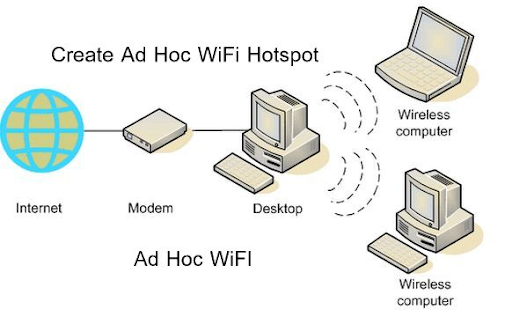
\includegraphics[scale=0.2]{adhoc.png}
    \caption{Exemplo de rede \textit{ad hoc}.}
    \label{01_model_graph}
\end{figure}

Uma rede \textit{ad hoc} pode ser modelada em um grafo grafo $G(V,E)$, ondes os vértices $V$ representam os nós da rede e as arestas $E$ representam conexão entre os nós. No caso de uma rede sem fio haveria conexão de acordo com a distância entre os nós, um raio de abrangência da conexão.

O problema do subconjunto dominante para um grafo $G(V,E)$, determina que existe um conjunto $D$, onde $D \subseteq G$ tal que todo vértice $V$ está contido em $D$ ou possui uma aresta $E$ para algum $V \subset D$. Achar o conjunto dominante $D$ de cardinalidade mínima é um problema NP-completo amplamente estudado. E uma variação deste problema é adicionar a exigência de que todos os vértice contidos em $D$ possuam arestas $E$ entre si, ou seja, sejam conexos.

A variação conexa do problema do conjunto dominante mínimo determina que para todos o par de vértice $n, m \in D$ exista um caminho inteiramente em $D$ que una esses nós.

Sabendo que muitas das aplicações para este problema utilizam redes sem fio, é analisado em \cite{Jovanovic} instâncias que espalham os nós da rede sobre um domínio em $R^2$ e determina um raio $r$, nós que possuírem um distância entre si $d < r$ serão definidos como vizinhos, ou seja, possuem conexão.

\subsection{O Problema}

Uma formulação simples para o problema do subconjunto dominante mínimo (\textit{Mimumum Weighted Dominant Set}, MWDS é dada pelas equações em \ref{01_min}. Nessa formulação temos o conjunto de vizinhança $N[i]$ que representa todos os nós adjacentes à $i$, o conjunto $D_v$ que representa o conjunto de nós dominantes selecionado e $w_i$ representa o custo ou peso de cada nó.

\begin{eqnarray*}
    min \sum_{i \in V} w_i x_i \\
    s.t. \sum_{j \in N[i} x_j  \geq 1 ,\text{ }\text{ }\text{ }\text{ }\text{ }\text{ }\text{ } \forall i \in D_v \\
         x_i \in [0,1],\text{ }\text{ }\text{ }\forall i \in D_v \\
         N[i] = {i} \cup (j |(i,j) \in E)
    \label{01_min}
\end{eqnarray*}

 O problema do conjunto dominante mínimo em sua variação conexa (\textit{Mimumum Weighted Connex Dominant Set}, MWCDS) possui definição presente em \ref{01_min} somadas as restrições de \ref{02_connex}. Sendo $N_d[i]$ a parte da vizinhança de $i$ que faz parte do conjunto dominante e $N_{cd}[i]$ sendo todos os nós dominantes conectados à um nó $i$.
 
\begin{eqnarray*}
    x_i \text{  e  } x_k \in \text{ } D_v\text{ }\text{ }\text{ }\text{ }\\
    N_d[i] = \text{ }\text{ }\text{ }\text{ }\text{ }N[i] \cap D_v\text{ }\text{ }\text{ }\\
    N_{cd}[i] = N_d \cup N_{cd}[N_d[i]]\\
    x_i \in N_{cd}[k] \text{  e  } x_k \in N_{cd}[i]
    \label{02_connex}
\end{eqnarray*}

\section{Metodologia}
Inicialmente, estipulou-se os passos necessários para se construir boas soluções para o problema.

\begin{itemize}
    \item Selecionar nó inicial randômico para busca.
    
    \item Realizar seleção de nós articulação.
    
    \item Adicionar pontos através de uma heurística de construção, até que se obtenha um conjunto dominante.
    
    \subitem Utilizar mesma heurística para completar solução caso o conjunto dominante obtido não seja conexo.
    
    \item Utilizar de alguma metaheurística para melhorar solução obtida.
\end{itemize}

Os nós articulação de um Grafo são aqueles cuja conexão do grafo seria desfeita, dado um nó inicial. O algoritmo utilizado para determinar tais nós possui tempo linear, proposto por \cite{Hopcroft}. Primeiramente é realizada uma busca em profundidade à partir de um nó inicial, durante a busca constrói-se a árvore de busca em profundidade com todos os nós do grafo. Caso o nó raiz possua pelo menos dois "filhos" ele é um nó de articulação. Adicionalmente, todo nó $i \in V - \{ raiz \}$ é um nó articulação, se há um nó $j$ "filho" de $i$, onde não haja aresta de $j$ ou qualquer descendente de $i$ para um possível sucessor de $j$

Foi observado que quando se utiliza de meteheurísticas de busca local ou metaheurísticas populacionais, os passos são os mesmos para a criação de solução ou soluções. Á cada iteração o algoritmo possuirá 3 conjuntos de vértices:

\begin{itemize}
    \item \textbf{Dominante}: Suposição de subconjunto de nós dominantes $D$.
    
    \item \textbf{Dominado}: Nós na vizinhança $N[D] = D_m$
    
    \item \textbf{Não-dominado}: Nós do grafo que não estão na vizinhança do suposto nó dominante, $nD = V - ( D \cup D_m )$. Caso $nD = \emptyset$, então o conjunto $D$ proposto é realmente dominante.
\end{itemize}


Como heurística de construção para as suposições de conjuntos dominantes foram utilizados as heurísticas:

\begin{itemize}
    \item \textbf{Gulosa}: Aonde cada vértice possui um custo associado e sempre a adição de menor custo é efetuada.
    
    \item \textbf{Gulosa Randomizada}: Aonde o algoritmo possui um $\alpha \in [0,1]$ que representa a porcentagem de melhores adições que será aleatoriamente feita. Caso $\alpha \equals 0$, a heurística é totalmente Gulosa. E, caso $\alpha \equals 1$ a heurística é totalmente randômica.
    
    \item \textbf{Gulosa Randomizada Reativa}: Além de possuir um $\alpha$ atual esta heurística armazena uma lista de $\alpha$ de tamanho $n_\alpha$. A cada iteração de construção nesta heurística um $\alpha$ é aleatoriamente selecionado. Uma vez selecionado é observada a melhora do conjunto dominante e a probabilidade do $\alpha$ selecionado é alterada de acordo.
\end{itemize}

Para a heurística Gulosa Randomizada Reativa foi utilizada a estrutura de loteria para probabilidade. Em caso de melhora na solução o $\alpha$ selecionado ganha um "\textit{ticket}" a mais que os outros. Para investigar a influências das abordagens propostas para o problema do conjunto dominante o problema foi modelado no esquema de classes exibido em \ref{01_model_graph}.

\begin{figure}[!htbp]
    \centering
    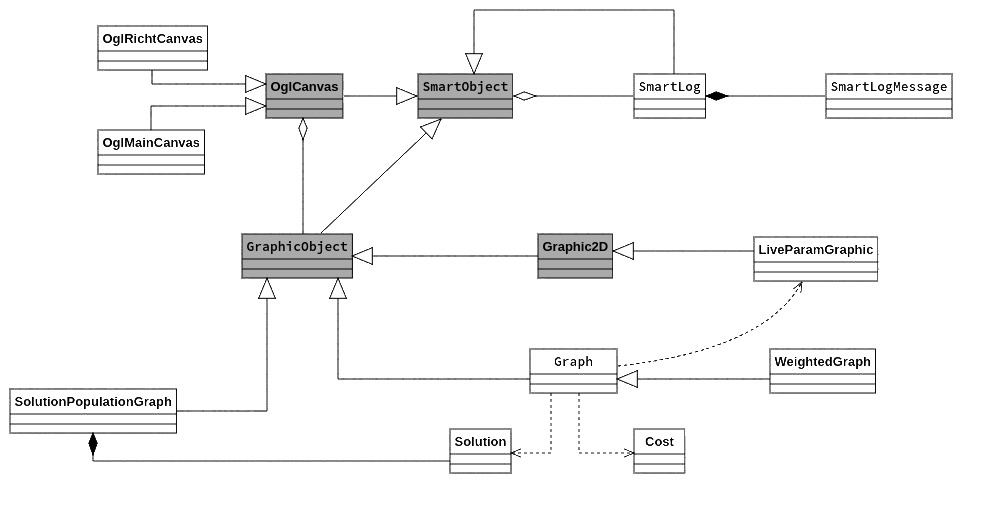
\includegraphics[scale=0.2]{ClassDiagram1_.jpg}
    \caption{Modelo de classes utilizado para as instâncias carregadas.}
    \label{01_model_graph}
\end{figure}

Este esquema de classes \textit{SmartObject} e \textit{GraphicObject} são provenientes do ferramenta computacional \textit{IGU}. Desta forma, todos os grafos que forem modelados neste esquema de classes pode ser manipulado pelo ambiente computacional. 

Na figura \ref{01_model_graph} estão em cinza as classes abstratas \textit{Graphic Object}, \textit{Smart Object}, \textit{OglCanvas} e \textit{Graphic2D}. Estas generalizações são apresentadas em \cite{Santos} para que um objeto e seus campos possam ser exibidos. Ainda na figura \ref{01_model_graph} vemos a classe \textit{Graph} que representa o modelo de grafo utilizado, como ele é uma generalização de um objeto gráfico ele pode se desenhar na tela. A generalização \textit{WeightedGraph} apresenta a modelagem feita para o MWCDS com pesos nas arestas e nos nós. As classes \textit{Solution} e \textit{Cost} representam uma soluções proposta para o problema e um custo atribuído à algum nó, respectivamente.

Um objeto da classe \textit{SolutionPopulationGraph} é composto por um vetor de soluções que pode representar a "população" de soluções para um dado grafo. Este objeto é utilizado para exibir na tela as diferentes soluções analisadas pelo algoritmo. As demais classes são provenientes de \cite{Santos}.

Esta modelagem permitiu que instâncias, como as de \cite{Jovanovic}, fossem carregadas e iteradas visualmente. O comportamento de cada heurística foi inserido na classe \textit{WeightedGraph} que pode mudar a estratégia para resolução em tempo de execução.

\begin{figure}[!htbp]
    \centering
    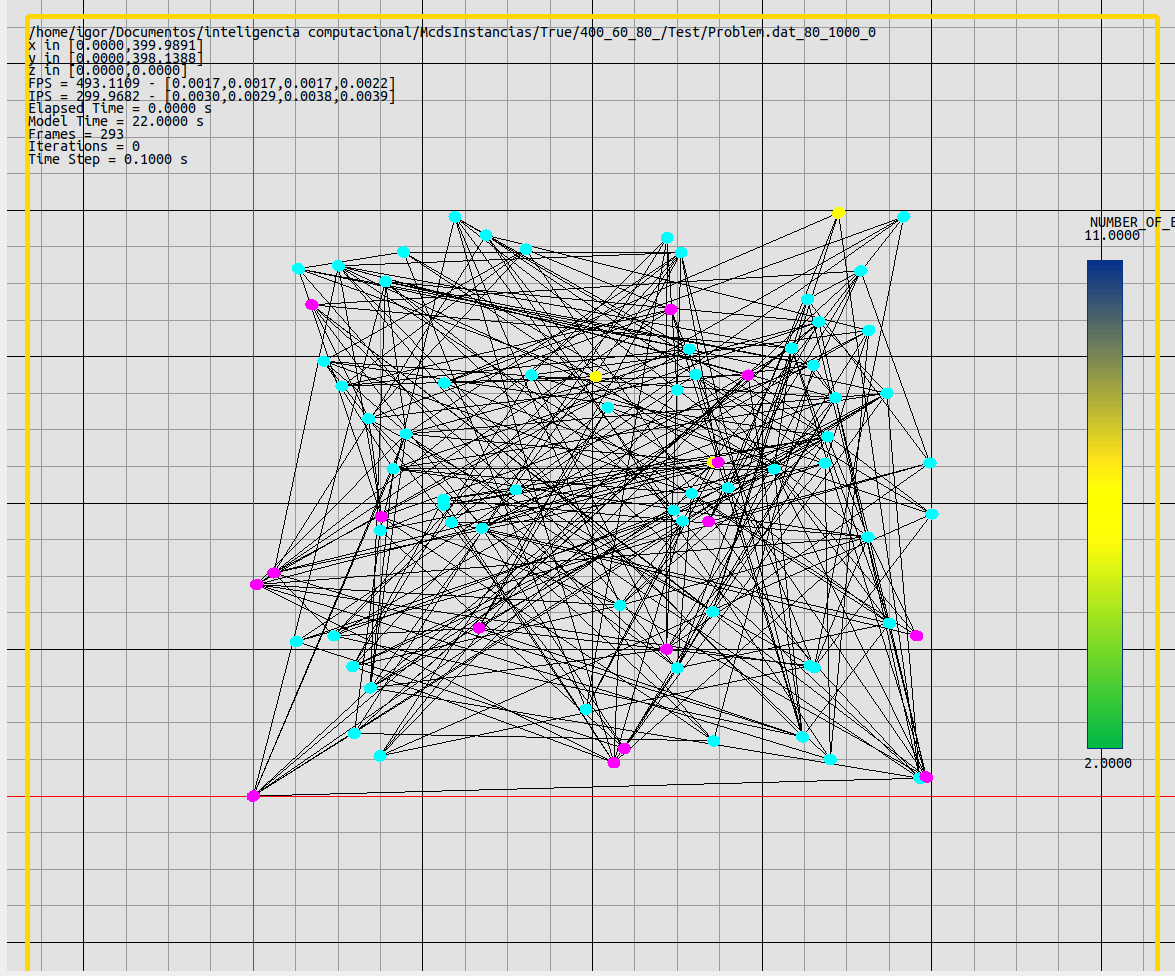
\includegraphics[scale=0.15]{IGU_SCREENSHOT__00005.png}
    \caption{Objeto \textit{WeightedGraph} carregado na ferramenta computacional \textit{IGU}. Em magenta os nós dominantes, em ciano os nós dominados e em amarelo os nós ainda não dominados.}
    \label{01_IGU}
\end{figure}

Uma vez carregado o objeto \textit{Graph} está sujeito à máquina de estados presente em \ref{01_model_graph}, que controla o comportamento do grafo.

\begin{figure}[!htbp]
    \centering
    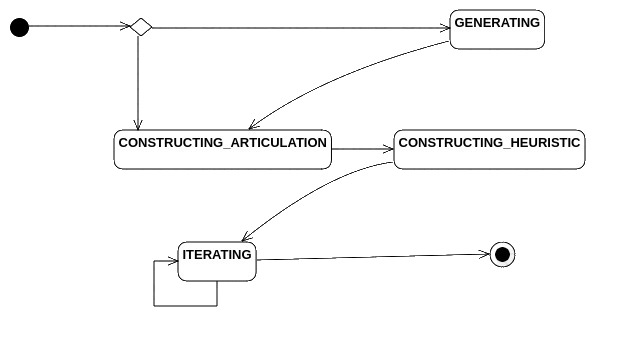
\includegraphics[scale=0.4]{GraphStatus_.jpg}
    \caption{Máquina de estados de \textit{Graph}}
    \label{01_graph_status}
\end{figure}

Quando carregado, o objeto inicia-se no estado \textit{CONSTRUCTING$\_$ARTICULATION} que é o estado em que supõe-se como conjunto dominante apenas os nós articulação dado algum nó randômico do grafo. No ambiente computacional existe também a possibilidade de se criar novos grafos randômicos para teste, neste caso os grafos são inicializados no estado \textit{GENERATING}, onde nós e arestas são adicionados até uma quantidade estipulada. E, caso o grafo gerado não seja conexo, mais arestas são adicionadas.

Durante a fase \textit{CONSTRUCTING$\_$HEURISTIC} as heurísticas de construção mencionadas anteriormente são utilizadas com alguma função de custo. Para este trabalho as seguintes funções de custo foram utilizadas:

\begin{itemize}
    \item \textbf{Peso}: O custo de cada nó $i$ é dado pelo seu peso $c_i$
    
    \subitem $w_i = c_i$
    
    \item \textbf{Conectividade}: O custo de cada nó $i$ é dado pelo inverso de sua conectividade $E_i$.
    
    \subitem $w_i = 1 / E_i$
    
    \item \textbf{Peso e Conectividade}: O custo de cada nó $i$ é dado pelo custo $c_i$ dividido por sua conectividade $E_i$.
    
    \subitem $w_i = c_i / E_i$
    
    \item \textbf{Dominância}: O custo de cada nó $i$ é dado pelo inverso de sua dominância $D_i$. A dominância é a quantidade de nós que a aresta possui na vizinhança que ainda não foram dominados.
    
    \subitem $w_i = 1 / D_i$
    
    \item \textbf{Peso e Dominância}: O custo de cada nó $i$ é dado pelo custo $c_i$ dividido por sua dominância $D_i$.
    
    \subitem $w_i = c_i / D_i$
\end{itemize}

Como o cálculo da dominância faz verificações de vizinhança estas funções possuem um custo computacional maior.

Uma vez que o grafo atinge o estado \textit{ITERATING} uma das metaheurísticas é selecionada e iterada. Para este trabalho foram implementadas as seguintes metaheurísticas:

\begin{itemize}
    \item \textbf{Metaheurísticas de Busca Local}
    
    \subitem \textbf{\textit{Variable Neighborhood Descent} (VND)}: Ao construir uma solução dominante e conexa, é analisada a vizinhança da solução e o primeiro aprimorante é selecionado, até que não haja mais melhora, então o grafo retorna ao estado \textit{CONSTRUCTING$\_$ARTICULATION} para reconstruir a solução. Isso é feito até que não haja melhora dada $N_{restart}$ reconstruções.
    
    \subitem \textbf{Tabu}: A busca Tabu recebe um solução por iteração e realiza algum movimento que não seja Tabu. Movimentos Tabu são adicionados para evitar que a busca local se torne cíclica e retorne aos mesmos resultados. Existe também um critério de aspiração que determina que se a solução gerada por um movimento Tabu possuir uma melhora maior que o critério de aspiração o movimento Tabu é realizado.
    
    \item \textbf{Metaheurística Populacional}
    
    \subitem \textbf{Colônia de Formigas}: A busca populacional Coônia de Formigas constrói um determinado número de soluções, determinadas "formigas". Desta forma as formigas são responsáveis por atualizar a sua solução de acordo com uma matriz de feromônios $\tau$ a atualizar esta matriz caso ocorra melhora na solução.
    
\end{itemize}

\subsection{Metaheurísticas de Busca Local}

As metaheurísticas de busca local levam em consideração todos os nós vizinhos à uma determinada solução. Como dito anteriormente, cada solução possui um conjunto de nós, a vizinhança de um solução é determinada através de soluções atingíveis com transformações neste conjunto de nós. As transformações utilizadas foram:

\begin{itemize}
    \item \textbf{Adicionar}: Dado um conjunto de vértices supostamente dominante $D$, adiciona-se qualquer nó $v \in V - D$ para criar um novo conjunto de soluções.
    
    \item \textbf{Remover}: Dado um conjunto de vértices supostamente dominante $D$, remove-se qualquer nó $v \in D$ para criar um novo conjunto de soluções.
    
    \item \textbf{Trocar}: Dado um conjunto de vértices supostamente dominante $D$ são analisadas as $\sqrt{\| D \|}$ melhores soluções dos movimentos adicionar e remover. Então faz-se a permutação das melhores remoções com as melhores adições, obtendo $\| D \|$ trocas possíveis. Assim como em \cite{Mayra};
\end{itemize}

Enfim a metaheurística constrói a vizinhança e decide como se movimentará.

\subsubsection{Variable Neighborhood Descent}

A metaheurística \textit{Variable Neighborhood Descent} (VND) consiste em construir diversas vizinhanças e movimentar-se sempre para o primeiro aprimorante. Isto significa que a heurística recebe uma solução com um subconjunto dominante, realiza movimentos que diminuam o seu custo final, ou seja, remove arestas. Seleciona àquele com menor custo final e quando não consegue mais uma solução possível com redução de custo, constrói uma nova solução.

Construir uma nova solução neste cenário consiste em voltar ao estado \textit{CONSTRUCTING$\_$ARTICULATION}, que construirá uma solução completamente nova.

A grande diferença do \textit{VND} é que esta metaheurística tenta aprimorar o valor de $\alpha$ utilizado na construção da seleção. O \textit{VND} funciona somente com o algoritmo construtivo reativo, pois assim como há reforço da probabilidade de $\alpha_n$ ao melhorar a solução no processo de construção, também há reforço ao melhorar a solução no processo de busca local, ou seja, cada vez que a solução possuir um vizinho de menor custo, um "\textit{ticket}" é adicionado à probabilidade do $\alpha$ utilizado para construir a solução. Assim a heurística tenta construir soluções melhores para o problema a cada iteração.

\subsubsection{Busca Tabu}

A metaheurística de busca considera as soluções alcançadas através de um movimento como vizinhança, exceto que no caso da busca tabu, as soluções não dominantes também serão analisadas e ranqueadas. Isso se dá através de um $\alpha_{penalisar}$. Primeiramente, consideramos como $S_0$ a solução inicial recebida pela busca tabu, que será dominante. Com base em $S$ e nas funções de custo apresentadas anteriormente como $W(S)$ se utiliza um cálculo de peso diferenciado, penalisando as soluções não possíveis:

\begin{eqnarray*}
    f(S) = W(S) + \alpha_{penalisar} * max(W(S)) * \| nD \|
    \label{01_min}
\end{eqnarray*}

Sendo $\| nD \|$ a quantidade de nós não dominados pela solução e $max(W(S))$ o peso máximo de um nó na solução. Esta metaheurística conta também com uma lista dos últimos movimentos, a lista tabu. Esta lista contém todos os movimentos que são considerados tabu, ou seja, são evitados. Isto é feito para evitar mínimos locais já atingidos, contudo isto tem um custo, que é o custo de armazenamento desta lista, para isto existe o parâmetro $N_{tabu}$.

Assim como o \textit{VND}, a busca tabu se movimenta para o primeiro aprimorante. Desde que o movimento não se encontre na lista tabu. Uma vez realizado o movimento, o seu oposto é incluído na lista tabu, isto é:

\begin{itemize}
    \item \textbf{Adicionar}: O movimento remover com o mesmo nó é incluído na lista tabu.
    
    \item \textbf{Remover}: O movimento adicionar com o mesmo nó é incluído na lista tabu.
    
    \item \textbf{Trocar}: O movimento adicionar com o nó removido e remover com o nó removido é incluído na lista tabu.
\end{itemize}

Contudo, ao analisar a vizinhança, se um movimento tabu for selecionado e possuir uma melhora maior que um critério de aspiração $\phi$ em relação a última solução iterada, o movimento é realizado mesmo sendo tabu. Visto em \cite{Mayra}, a busca tabu pode ser incrementada com uma perturbação em seus nós a cada $N_{perturbar}$ iterações e reconstrói uma solução. Reconstruir o grafo mais uma vez significa alterar o estado do objeto iterado para \textit{CONSTRUCTING$\_$HEURISTIC}, aonde o grafo irá adicionar nós à solução de acordo com algum algoritmo de construção mencionado anteriormente.

Isto é feito até atingir o máximo de iterações sem melhora $\phi_best$.

\subsection{Metaheurística Populacional}

Em seguida foi proposta uma metaheurística populacional para o problema, no caso a colônia de formigas (\textit{Ant Colony Optmization}, ACO) foi escolhida para o problema. Algoritmo este apresentado em \cite{Jovanovic} com o conceito de feromônios, reforçando boas qualidades que "evaporam" com o tempo.

Assim como as metaheurísticas  de busca local, a colônia de formigas recebe uma solução ao começo de sua execução, a sua diferença é que esta solução é armazenada e chamada de "formiga", pois ela será responsável por reforçar feromônios e caminhas sobre eles. Uma vez armazenada a solução, novas soluções são geradas retornando o grafo para o estado \textit{CONSTRUCTING$\_$ARTICULATION} e ao chegar no estado \textit{ITERATING} a solução é armazenada em um vetor até que se chegue ao tamanho desejado $N_{ants}$.

Como mencionado anteriormente, esta heurística utiliza de feromônios para reforçar boas qualidades na solução. Para isto utilizamos um vetor $\tau^0$ para cada formiga que contém os feromônios correspondentes à sua primeira solução $S_0$.

\begin{eqnarray*}
    \tau_i^0 = \begin{cases} 
                0, & \mbox{se } i \notin D\\ 
                \frac{1}{\| D\|}, & \mbox{se } i \in D
                \end{cases}
    \label{01_ants}
\end{eqnarray*}

Precisamos também de um vetor $\tau_i$ que armazena o feromônio armazenado em cada vértice $i$. O vetor$\tau_i$ inicialmente recebe o valor do primeiro $\tau_0$. E, a cada melhora da solução global atualiza $\tau_i$ seguindo \ref{02_ants}.

\begin{eqnarray*}
    \tau_i = (1 - p) \tau_i + \delta\tau_i
    \label{02_ants}
\end{eqnarray*}

Onde $p$ é o grau de evaporação e $\delta\tau_i$ é calculado como \ref{03_ants}.

\begin{eqnarray*}
    \delta\tau_i = \begin{cases} 
                0, & \mbox{se } i \notin D\\ 
                \frac{1}{\| D\|}, & \mbox{se } i \in D
                \end{cases}
    \label{03_ants}
\end{eqnarray*}

E, finalmente temos um vetor local $\tau_i^{'}$ para cada formiga com a sua quantidade de feromônios, este vetor é atualizado também à cada iteração.

\begin{eqnarray*}
    \tau_i^{'} = (1 - \phi) \tau_i + \phi \tau^0_i
    \label{02_ants}
\end{eqnarray*}

Assim os feromônios da colônia de formigas são definidos. À cada iteração existirá este cálculo de feromônios e a heurística então criará as $N_{ants}$ atualizando seus feromônios. Uma vez construídas, as formigas entrarão em uma busca primeiro-aprimorante, assim como a VND para diminuir o custo da primeira solução com uma busca simples. Quando não houverem mais vizinhos aprimorantes a solução é perturbada em $pert$ por cento, aonde $pert$ é um número randômico para cada formiga.

Uma vez perturbadas as soluções precisam adicionar nós seguindo os feromônios $\tau_i$, para isto construímos o vetor $prob_i$.

\begin{eqnarray*}
    prob_i =  \begin{cases} 
                0, & \mbox{se } q > q_0  \mbox{ e } i \neq argmax \frac{\tau_i}{w_i}\\ 
                1, & \mbox{se } q > q_0 i \mbox{ e } i = argmax \frac{\tau_i}{w_i}\\ 
                \frac{\frac{\tau_i}{w_i}}{\sum\frac{\tau_i}{w_i}}, & \mbox{se } q \leq q_0
                \end{cases}
    \label{03_ants}
\end{eqnarray*}

Onde $w_i$ segue alguma das funções de custo mencionadas anteriormente, $q_0$ a taxa de exploração que determina o quanto deve-se explorar o nó com feromônio mais forte e $q$ um número randômico. Sendo que $q$ e $q_0 \in [0,1]$.

Então adicionam-se nós a solução até que se tenha uma solução possível. Quando se obtêm uma solução possível uma nova busco local primeiro-aprimorante é feita. Estes passo são realizados até atingir o máximo de iterações sem melhora $\phi_best$.


\section{Desenvolvimento}

Como mencionado anteriormente o objeto gráfico que representa um grafo é denominado \textit{WeightedGraph}. Assim como todos os objetos carregados na ferramenta computacional, ele é exibido e iterado simultaneamente.

O objeto é capaz de se desenhar através de diretivas \textit{OpenGL} \cite{OpenGL}, que utiliza ponteiros para as seus dados que informam a cor de cada nó. Isto é feito inicialmente ao carregar um objeto gŕafico, quando sua parâmetros visuais e iniciais são definidos.

\begin{algorithm}
\caption{Inicialização}\label{iteration}
\begin{algorithmic}[1]
\Procedure{Initialize}{}
  $carregaParâmetrosVisuais()$
  $carregaParâmetrosIniciais()$
  
    \If {$conexo \textit{or} N > MINIMO$} 
        \State $\textit{estadoGrafo} \gets \text{GENERATING}$
    \EndIf
  
\EndProcedure
\end{algorithmic}
\end{algorithm}

Em \ref{iteration} os parâmetros visuais representam aqueles que fazem alguma diferença quanto a visualização, já os parâmetros iniciais remetem à todos os parâmetros mencionados na seção 2, bem como quais heurísticas utilizar.

Uma outra \textit{thread} é alocada para simultaneamente iterar este objeto. Uma iteração do objeto \textit{WeightedGraph} é determinada pelo seguinte algoritmo.

\begin{algorithm}
\caption{Iteração}\label{iteration}
\begin{algorithmic}[1]
\Procedure{Iteration}{}
  \Switch{$estadoGrafo$}
    \Case{$GENERATING$}
    
    \State $\textit{nós +=} \textit{randomNodes}()$
    
    \If {$conexo && N > MINIMO$} 
        \State $\textit{estadoGrafo} \gets \text{CONSTRUCTING\_ARTICULATION}$
    \EndIf
    \EndCase
    \Case{$CONSTRUCTING\_ARTICULATION$}
      \State $\textit{ultimaSolução = } \textit{articulação}()$
      
      \State $\textit{estadoGrafo} \gets \text{CONSTRUCTING\_HEURISTIC}$
    \EndCase
    \Case{$CONSTRUCTING\_HEURISTIC$}
      \State $\textit{ultimaSolução += adicionaNó}(\textit{heurísticaConstrutiva})$
      
    
    \If {$ultimaSolução.conexo \textit{ \&\& } ultimaSolução.dominante$} 
        \State $\textit{estadoGrafo} \gets \text{ITERATING}$
    \EndIf
    \EndCase
    \Case{$ITERATING$}
        \Switch{$\textit{heurísticaIteração}$}
        \EndSwitch
    \EndCase
  \EndSwitch
\EndProcedure
\end{algorithmic}
\end{algorithm}

Dentro do estado \textit{ITERATING} observa-se uma funcionalidade diferente para cada heurística de iteração selecionada, estas são as heurísticas de busca local e a heurística populacional (VND, Busca Tabu e Colônia de Formigas).

\section{Resultados}

Nesta seção estão os resultados obtidos com as heurísticas descritas. O custo considerado foi a conectividade do vértice, que foi o mais rápido e com melhores resultados iniciais. As instâncias foram carregadas automaticamente utilizando o ambiente computacional \textit{IGU} e testadas, gerando os seguintes relatórios.

Os resultados aqui exibidos foram obtidos em uma máquina equipada com um processador Intel(R) Core(TM) i9-9900K CPU @ 3.60GHz, possuindo 8 núcleos e 16 threads, conectados à 16GB de Memória RAM 3000MHz. Os parâmetros utilizados em cada objeto carregado foram:

\begin{itemize}
    \item \textbf{Parâmetros gerais}: parâmetros que afetam todas as instâncias.
    
        \subitem \textbf{Desenho}: desativa o desenho de cada instância para que obtenha um desempenho maior.
    
        \subitem \textbf{Custo}: determina qual critério deve ser utilizado para definir o custo de cada nó. Em todos os testes realizados as instâncias obtiveram melhor resultado utilizando o inverso da quantidade de vértices.
    
        \subitem \textbf{Heurística construtiva}: determina qual heurística deve ser utilizada para se construir a primeira solução. Em todos os testes realizados as instâncias obtiveram melhores resultados utilizando a heurística gulosa construtiva randomizada reativa.
    
        \subitem \textbf{Movimentos considerados}: determina quais movimentos devem ser considerados para se construir a vizinhança. Em todos os testes realizados as instâncias obtiveram melhores resultados utilizando os movimentos de adição, remoção e troca de nós.
    
    \item \textbf{Parâmetros VND}: parâmetros que afetam todas as instâncias que usarem a heurística VND.
    
        \subitem \textbf{Quantida de de repetições}: determina a quantidade de soluções que devem ser construídas e analisadas. Em todos os testes realizados as instâncias obtiveram melhores resultados utilizando $N_{repete} = 1000$.
    
    \item \textbf{Parâmetros busca tabu}: parâmetros que afetam todas as instâncias que usarem a heurística busca tabu.
    
        \subitem \textbf{Alfa de penalização}: determina o máximo, o mínimo e tamanho do ciclo do alfa penalização. Em todos os testes realizados as instâncias obtiveram melhores resultados utilizando $\alpha_{max} = 1.1, \alpha_{min} = 0.1, N_{\alpha} = 25$.
    
        \subitem \textbf{Tamanho da lista tabu}: determina o tamanho da lista tabu, ou seja, movimentos que serão descartados. Em todos os testes realizados as instâncias obtiveram melhores resultados utilizando $N_{tabu} = 12$.
    
        \subitem \textbf{Iterações até a repetição}: determina a quantia de de iterações que devem ser feitas até perturbar-se a solução. Em todos os testes realizados as instâncias obtiveram melhores resultados utilizando $N_{perturbate} = 100$.
    
    \item \textbf{Parâmetros colônia de formigas}: parâmetros que afetam todas as instâncias que usarem a heurística colônia de formigas.
    
        \subitem \textbf{Tamanho da colônia}: determina o o tamanho da colônia de formigas, ou seja, a quantidade de soluções que são analisadas simultaneamente. Em todos os testes realizados as instâncias obtiveram melhores resultados, sem comprometer demais o tempo de cada iteração, utilizando $N_{ants} = 24$.
    
        \subitem \textbf{Força da trilha de feromônio}: determina a força com que deve-se alterar a matriz de feromônios à cada melhora na solução. Em todos os testes realizados as instâncias obtiveram melhores resultados utilizando $p = 0.9$.
    
        \subitem \textbf{Força do feromônio local}: determina a força com que deve-se alterar a solução. Em todos os testes realizados as instâncias obtiveram melhores resultados utilizando $\phi = 0.9$.
    
        \subitem \textbf{Taxa de exploração}: determina o quanto cada "formiga" deve seguir a trilha de feromônios ou exploras novas soluções. Em todos os testes realizados as instâncias obtiveram melhores resultados utilizando $q0 = 0.9$.
    
\end{itemize}

As instâncias foram extraídas de \cite{Jovanovic}.

\section{Conclusão}

As heurísticas obtiveram resultados similares ao esperado. O código gerado é aberto e se encontra no repositório aberto:

\centering{\textit{http://bit.ly/2KwZ4np}}

Menciona-se também que os resultados extraídos da literatura obtiveram um funcionamento próximo ao esperado. O algoritmo \textit{Variables Descent Neighboor} obteve os piores resultados gerais, pois obtêm muito pouca informação de sua vizinhança. O VND é uma heurística que se baseia totalmente em probabilidades e na heurística de construção utilizada.

Já a metaheurística de busca Tabu é capaz de navegar pela vizinhança e obter informações na tentativa de obter os mais diversos mínimos locais através da sua lista de movimentos tabu. Ao comparar os resultados obtidos desta heurística com os resultados obtidos em \cite{Mayra}, observamos uma distanciação dos melhores resultados grande, que nas maiores instâncias chega à 120\%. Estima-se que este erro foi induzido nos parâmetros da busca tabu, como quantidade de iterações até a perturbação e até a heurística utilizada para perturbar a solução. Entretanto, a heurística agiu como o esperado.

Por último, a metaheurística populacional de colônia de formigas visitou à vizinhança de forma diferente. Nos resultados aqui descritos comenta-se que os resultados da colônia de formigas obtiveram maior acurácia e precisão do que a busca Tabu, variando seu resultado menos que todas as outras heurísticas comparadas. Entretanto foi também a heurística que mais exigiu poder computacional, trabalhando à todo tempo com 24 soluções em memória e visitando suas vizinhanças.

A ferramenta serviu para guiar e possibilitar a análise dos grafos através de diferentes visualizações. O que facilitou alterações no código e definição da acurácia.

Futuramente, pretende-se aumentar a quantidade de algoritmos suportados para verificar em um mesmo ambiente a melhora tanto na solução quanto no tempo computacional.

\newpage
\newpage
\clearpage

\begin{adjustbox}{angle=90,width={\textwidth},totalheight={22cm},keepaspectratio,caption={Tabela de Resultados},center={14cm}}
% \begin{table}
\begin{tabular}{|l|l|l|l|l|l|l|l|l|l|l|l|l|l|l|l|}
\hline
\multicolumn{1}{|c|}{\multirow{2}{*}{\textbf{Área}}} & \multicolumn{1}{c|}{\multirow{2}{*}{\textbf{N}}} & \multicolumn{1}{c|}{\multirow{2}{*}{\textbf{Raio}}} & \multicolumn{4}{c|}{\textbf{VND}}                                           & \multicolumn{4}{c|}{\textbf{Tabu}}                                          & \multicolumn{4}{c|}{\textbf{Colônia de Formigas}}                           & \multirow{2}{*}{\textbf{Melhor}} \\ \cline{4-15}
\multicolumn{1}{|c|}{}                               & \multicolumn{1}{c|}{}                            & \multicolumn{1}{c|}{}                               & \textbf{Melhor} & \textbf{Média} & \textbf{Gap Melhor} & \textbf{Gap Média} & \textbf{Melhor} & \textbf{Média} & \textbf{Gap Melhor} & \textbf{Gap Média} & \textbf{Melhor} & \textbf{Média} & \textbf{Gap Melhor} & \textbf{Gap Média} &                                  \\ \hline
\textbf{400}                                         & \textbf{80}                                      & \textbf{60}                                         & 20,0            & 21,3           & 11,1\%              & 18,3\%             & 20,0            & 33,6           & 11,1\%              & 86,7\%             & 20,0            & 26,6           & 11,1\%              & 47,8\%             & 18                               \\ \hline
\textbf{}                                            & \textbf{80}                                      & \textbf{70}                                         & 16,0            & 24,9           & 14,3\%              & 78,0\%             & 16,0            & 26,0           & 14,3\%              & 86,0\%             & 15,0            & 25,4           & 7,1\%               & 81,8\%             & 14                               \\ \hline
\textbf{}                                            & \textbf{80}                                      & \textbf{80}                                         & 14,0            & 15,6           & 16,7\%              & 29,8\%             & 14,0            & 21,8           & 16,7\%              & 81,3\%             & 13,0            & 20,9           & 8,3\%               & 73,9\%             & 12                               \\ \hline
\textbf{}                                            & \textbf{80}                                      & \textbf{90}                                         & 12,0            & 13,1           & 20,0\%              & 30,8\%             & 12,0            & 16,0           & 20,0\%              & 60,2\%             & 11,0            & 18,7           & 10,0\%              & 86,6\%             & 10                               \\ \hline
\textbf{}                                            & \textbf{80}                                      & \textbf{10}                                         & 9,0             & 12,0           & 12,5\%              & 49,6\%             & \textbf{8,0}    & \textbf{19,8}  & \textbf{0,0\%}      & \textbf{147,0\%}   & \textbf{8,0}    & \textbf{16,9}  & \textbf{0,0\%}      & \textbf{111,2\%}   & 8                                \\ \hline
\textbf{}                                            & \textbf{80}                                      & \textbf{110}                                        & 9,0             & 11,0           & 28,6\%              & 56,6\%             & 8,0             & 12,5           & 14,3\%              & 78,6\%             & 9,0             & 29,8           & 28,6\%              & 325,1\%            & 7                                \\ \hline
\textbf{}                                            & \textbf{80}                                      & \textbf{120}                                        & 8,0             & 9,7            & 33,3\%              & 61,2\%             & 6,0             & 13,4           & 0,0\%               & 123,4\%            & 7,0             & 30,1           & 16,7\%              & 402,3\%            & 6                                \\ \hline
\textbf{600}                                         & \textbf{100}                                     & \textbf{80}                                         & 27,0            & 29,7           & 28,6\%              & 41,5\%             & 29,0            & 44,9           & 38,1\%              & 113,9\%            & 23,0            & 35,7           & 9,5\%               & 70,2\%             & 21                               \\ \hline
\textbf{}                                            & \textbf{100}                                     & \textbf{90}                                         & 25,0            & 27,6           & 31,6\%              & 45,2\%             & 25,0            & 35,4           & 31,6\%              & 86,1\%             & 22,0            & 33,6           & 15,8\%              & 76,6\%             & 19                               \\ \hline
\textbf{}                                            & \textbf{100}                                     & \textbf{100}                                        & 20,0            & 25,1           & 25,0\%              & 57,1\%             & 21,0            & 36,5           & 31,3\%              & 128,4\%            & 18,0            & 35,4           & 12,5\%              & 121,5\%            & 16                               \\ \hline
\textbf{}                                            & \textbf{100}                                     & \textbf{110}                                        & 17,0            & 21,0           & 21,4\%              & 49,7\%             & 17,0            & 27,1           & 21,4\%              & 93,4\%             & 16,0            & 32,7           & 14,3\%              & 133,2\%            & 14                               \\ \hline
\textbf{}                                            & \textbf{100}                                     & \textbf{120}                                        & 16,0            & 20,8           & 23,1\%              & 59,8\%             & 16,0            & 26,3           & 23,1\%              & 102,6\%            & 14,0            & 28,9           & 7,7\%               & 122,6\%            & 13                               \\ \hline
\textbf{700}                                         & \textbf{200}                                     & \textbf{70}                                         & 65,0            & 110,7          & 71,1\%              & 191,4\%            & 62,0            & 179,7          & 63,2\%              & 373,0\%            & 69,0            & 111,6          & 81,6\%              & 193,7\%            & 38                               \\ \hline
\textbf{}                                            & \textbf{200}                                     & \textbf{80}                                         & 56,0            & 123,4          & 75,0\%              & 285,6\%            & 50,0            & 150,8          & 56,3\%              & 371,2\%            & 56,0            & 107,7          & 75,0\%              & 236,6\%            & 32                               \\ \hline
\textbf{}                                            & \textbf{200}                                     & \textbf{90}                                         & 42,0            & 95,2           & 61,5\%              & 266,3\%            & 37,0            & 159,1          & 42,3\%              & 512,0\%            & 41,0            & 105,2          & 57,7\%              & 304,7\%            & 26                               \\ \hline
\textbf{}                                            & \textbf{200}                                     & \textbf{100}                                        & 35,0            & 87,8           & 59,1\%              & 298,9\%            & 34,0            & 150,0          & 54,5\%              & 581,9\%            & 30,0            & 95,2           & 36,4\%              & 332,9\%            & 22                               \\ \hline
\textbf{}                                            & \textbf{200}                                     & \textbf{110}                                        & 31,0            & 75,9           & 55,0\%              & 279,5\%            & 29,0            & 104,2          & 45,0\%              & 420,9\%            & 29,0            & 68,1           & 45,0\%              & 240,3\%            & 20                               \\ \hline
\textbf{}                                            & \textbf{200}                                     & \textbf{120}                                        & 26,0            & 80,6           & 52,9\%              & 373,9\%            & 25,0            & 216,3          & 47,1\%              & 1172,2\%           & 22,0            & 70,7           & 29,4\%              & 315,9\%            & 17                               \\ \hline
\textbf{1000}                                        & \textbf{200}                                     & \textbf{100}                                        & 67,0            & 111,0          & 76,3\%              & 192,2\%            & 66,0            & 205,8          & 73,7\%              & 441,5\%            & 57,0            & 118,4          & 50,0\%              & 211,6\%            & 38                               \\ \hline
\textbf{}                                            & \textbf{200}                                     & \textbf{110}                                        & 55,0            & 124,1          & 61,8\%              & 265,0\%            & 54,0            & 173,7          & 58,8\%              & 411,0\%            & 58,0            & 118,8          & 70,6\%              & 249,5\%            & 34                               \\ \hline
\textbf{}                                            & \textbf{200}                                     & \textbf{120}                                        & 47,0            & 101,4          & 62,1\%              & 249,5\%            & 46,0            & 224,2          & 58,6\%              & 673,0\%            & 43,0            & 95,9           & 48,3\%              & 230,6\%            & 29                               \\ \hline
\textbf{}                                            & \textbf{200}                                     & \textbf{130}                                        & 44,0            & 65,1           & 69,2\%              & 150,3\%            & 43,0            & 133,5          & 65,4\%              & 413,3\%            & 37,0            & 93,7           & 42,3\%              & 260,5\%            & 26                               \\ \hline
\textbf{}                                            & \textbf{200}                                     & \textbf{140}                                        & 37,0            & 72,0           & 60,9\%              & 213,2\%            & 40,0            & 125,4          & 73,9\%              & 445,2\%            & 32,0            & 92,2           & 39,1\%              & 301,0\%            & 23                               \\ \hline
\textbf{}                                            & \textbf{200}                                     & \textbf{150}                                        & 36,0            & 65,2           & 71,4\%              & 210,3\%            & 32,0            & 90,9           & 52,4\%              & 333,0\%            & 30,0            & 94,4           & 42,9\%              & 349,5\%            & 21                               \\ \hline
\textbf{}                                            & \textbf{200}                                     & \textbf{160}                                        & 31,0            & 69,7           & 63,2\%              & 266,8\%            & 29,0            & 123,3          & 52,6\%              & 549,1\%            & 23,0            & 92,5           & 21,1\%              & 387,0\%            & 19                               \\ \hline
\textbf{1500}                                        & \textbf{250}                                     & \textbf{130}                                        & 95,0            & 223,4          & 93,9\%              & 355,9\%            & 91,0            & 226,3          & 85,7\%              & 361,8\%            & 103,0           & 157,4          & 110,2\%             & 221,2\%            & 49                               \\ \hline
\textbf{}                                            & \textbf{250}                                     & \textbf{140}                                        & 82,0            & 108,7          & 86,4\%              & 147,0\%            & 86,0            & 196,6          & 95,5\%              & 346,9\%            & 73,0            & 127,2          & 65,9\%              & 189,0\%            & 44                               \\ \hline
\textbf{}                                            & \textbf{250}                                     & \textbf{150}                                        & 74,0            & 107,6          & 85,0\%              & 169,0\%            & 76,0            & 240,5          & 90,0\%              & 501,2\%            & 63,0            & 122,6          & 57,5\%              & 206,5\%            & 40                               \\ \hline
\textbf{}                                            & \textbf{250}                                     & \textbf{160}                                        & 70,0            & 112,3          & 94,4\%              & 212,0\%            & 71,0            & 205,4          & 97,2\%              & 470,6\%            & 59,0            & 118,8          & 63,9\%              & 229,9\%            & 36                               \\ \hline
\textbf{2000}                                        & \textbf{300}                                     & \textbf{200}                                        & 85,0            & 190,1          & 102,4\%             & 352,6\%            & 90,0            & 419,7          & 114,3\%             & 899,3\%            & 75,0            & 155,0          & 78,6\%              & 269,1\%            & 42                               \\ \hline
\textbf{}                                            & \textbf{300}                                     & \textbf{210}                                        & 74,0            & 164,9          & 89,7\%              & 322,7\%            & 80,0            & 269,6          & 105,1\%             & 591,3\%            & 66,0            & 159,9          & 69,2\%              & 310,0\%            & 39                               \\ \hline
\textbf{}                                            & \textbf{300}                                     & \textbf{220}                                        & 72,0            & 188,8          & 105,7\%             & 439,4\%            & 77,0            & 266,0          & 120,0\%             & 659,9\%            & 68,0            & 177,2          & 94,3\%              & 406,2\%            & 35                               \\ \hline
\textbf{}                                            & \textbf{300}                                     & \textbf{230}                                        & 66,0            & 195,9          & 100,0\%             & 493,7\%            & 70,0            & 431,6          & 112,1\%             & 1207,9\%           & 64,0            & 175,7          & 93,9\%              & 432,3\%            & 33                               \\ \hline
\end{tabular}
% \end{table}
\end{adjustbox}
 
\newpage
\clearpage
\newpage






% trigger a \newpage just before the given reference
% number - used to balance the columns on the last page
% adjust value as needed - may need to be readjusted if
% the document is modified later
%\IEEEtriggeratref{8}
% The "triggered" command can be changed if desired:
%\IEEEtriggercmd{\enlargethispage{-5in}}

% references section

% can use a bibliography generated by BibTeX as a .bbl file
% BibTeX documentation can be easily obtained at:
% http://mirror.ctan.org/biblio/bibtex/contrib/doc/
% The IEEEtran BibTeX style support page is at:
% http://www.michaelshell.org/tex/ieeetran/bibtex/
%\bibliographystyle{IEEEtran}
% argument is your BibTeX string definitions and bibliography database(s)
%\bibliography{IEEEabrv,../bib/paper}
%
% <OR> manually copy in the resultant .bbl file
% set second argument of \begin to the number of references
% (used to reserve space for the reference number labels box)
\begin{thebibliography}{1}

\bibitem{Mayra}
Mayra Carvalho Albuquerque, Matheuristics for Variants of the
Dominating Set Problem, Rio de janeiro, Brasil: Tese de Doutorado PUC-Rio, 2018.

\bibitem{Jovanovic}
Raka Jovanovic and Milan Tuba, Ant Colony Optimization Algorithm
with Pheromone Correction Strategy for
the Minimum Connected Dominating Set Problem, Harlow, England: Addison-Wesley, 2013.

\bibitem{Santos}
Igor Pires dos Santos, Modelagem e simulação de escoamento
sanguı́neo em árvores arteriais,Juiz de Fora, Brasil: Trabalho de Conclusão de Curso Engenharia Computacional - UFJF, 2019.

\bibitem{Hopcroft}
Hopcroft, J. & Tarjan, R.  Algorithm 447: efficient algorithms for graph
manipulation, Communications of the ACM 16(6), 372–378, 1973.

\bibitem{OpenGL}
Khronos Group. \site{www.opengl.org} , 2019.

\bibitem{VND}
Hansen, P., Mladenović, N. & Moreno Pérez, J.A. Ann Oper Res (2010) 175: 367. https://doi.org/10.1007/s10479-009-0657-6

\end{thebibliography}




% that's all folks
\end{document}


